\documentclass{article}
\usepackage{float}
\usepackage{graphicx}
\author{Simone Abelli, Stefano Azzone}
\title{DIMA Project report: MBox}
\begin{document}
\maketitle
\newpage
\tableofcontents
\newpage
\section{Introduction}
\subsection{Purpose}
The purpose of this document is to provide more technical and detailed
information about the mobile application developed. The Design Document is a
guide for the programmer that will manage the future development of the codebase
for the application in all its functions. The document will explain and motivate
all the architectural choices by providing a description of the components and
their interaction. We will also enforce the quality of the product through a set
of design characteristics. Finally we describe the implementation, integration
and test planning.
The topics touched by this document are:
\begin{itemize}
	\item high level architecture
	\item main components, screens and widgets
	\item runtime behavior
	\item design patterns
	\item more details on user interface
	\item requirements and their mapping on the architecture
	\item implementation and test planning
\end{itemize}

\subsection{Scope}
MBox is an application for mobile devices that allows users to access all the
music present on their devices without having to worry about manually managing 
the metadata. The target user has basic knowledge of the functions of the
mobile device (e.g. is able to interact with the filesystem). Since the
application is focused on users who want to listen to music, which is usually
done with a portable device, we will focus smartphones maily (the application
also works on tablets). For the development of this applications we have decided
to use flutter since it's a framework thought for multiplatform deployment.

\subsection{Glossary}
\paragraph{Queue:} a queue is a data structure containing a list of tracks
which are to be played according to a FIFO policy.
\paragraph{Metadata: } metadata are information of a track regarding the track
itself (e.g. track title, artist, album cover \ldots)

\newpage

\section{Description and requirements}
\subsection{Product description}
MBox has all the functionalities of a music player:
\begin{itemize}
    \item Detect music present in the Music folder
    \item Allow management of playlists
    \item Organize music by artist, album and playlist
    \item Allow to arrange tracks in a playback queue
    \item Play tracks (in random order if desired)
    \item Visualize metadata related to tracks
\end{itemize}
In addition to this, MBox allows a more advanced and automated metadata
management, and the access to other music information:
\begin{itemize}
    \item Automatically set missing metadata (Title, Artist, Album, Cover,
        Lyrics, Track number, Artist image, \ldots)
    \item Manually edit metadata
    \item Visualize information about artists like a brief description, albums
        and other songs
    \item Search on the internet for other songs and listen to them
\end{itemize}

\subsection{Assumptions}
\begin{itemize}
    \item When downloading metadata or looking for other music, internet
        connection is available
    \item The user is able to move their music to the Music folder
    \item The tracks are present on Spotify to download metadata
    \item When the user looks for a track not present on their device, it must
        be present on YouTube
    \item The tracks are in mp3 format (otherwise metadata management is harder)
    \item The access to the filesystem is granted
    \item The device on which the application is used has some means to 
        play music
\end{itemize}

\subsection{Functional requirements}
\begin{enumerate}
    \item The application can access the filesystem and fetch songs from the
        music folder
    \item The application can play the selected tracks
    \item The application allows the user to add or remove tracks from the
        playback queue
    \item The application allows the user to pause and resume playback
    \item The application allows the user to skip tracks in the queue
    \item The application should save the queue state to resume playback if the
        application is closed
    \item The application allows the user to add or remove playlists
    \item The application allows the user to add or remove tracks from playlists
    \item The application organizes the tracks by artist and album
    \item The application allows the user to view lyrics of currently playing 
        track
    \item The application allows the user to edit metadata of the tracks
    \item The application automatically adds missing metadata using an external
        service (in our case Spotify); already present metadata is kept
    \item The application can show information about the artists of the tracks
        present on the device (such as all their albums and tracks)
    \item The application allows the user to search for tracks not present on
        their device, and play them through an external service (in our case
        YouTube)
    \item It should be possible to use the application without an internet
        connection, obviously with limited functionalities (no external song
        search, metadata editing \ldots)
\end{enumerate}

\subsection{Non functional requirements}
\begin{enumerate}
    \item The application should feel snappy and responsive
    \item The application layout should be intuitive to use
    \item The application should be reliable
\end{enumerate}
\newpage

\section{Architectural Design}
\subsection{Architectural Style}
The application is logically subdivided in a frontend and a backend.
The frontend presents the information to the user and allows them to interact
with the backend. The backend contains and manages all the data and interfaces
with the external services.
\subsubsection{Frontend}

\begin{figure}[H]
	\noindent
	\makebox[\textwidth]{ 
		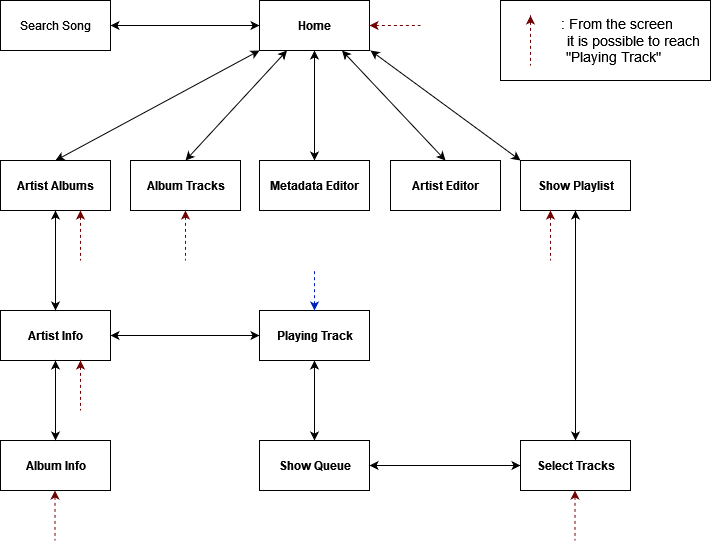
\includegraphics[scale=0.6]{images/ScreensDiagram.png}}
	\caption{Frontend system architecture} 
\end{figure}

The frontend is composed by the screens of the application. Once opened MBox
shows the \textbf{Home} screen. The Home screen is composed by 4 tabs:
\begin{itemize}
    \item \textit{Tracks}: a list of the tracks in alphabetical order; by
        selecting one we switch to the \textbf{PlayingTrack} screen, and start
        playing that track.
    \item \textit{Albums}: a list of the albums in alphabetical order; by
        selecting one we switch to the \textbf{AlbumTracks} screen, where we can
        select a track to play. 
    \item \textit{Artists}: a list of the artists in alphabetical order; by
        selecting one we switch to the \textbf{AlbumArtists} screen, where  we
        can select an album to show.
    \item \textit{Playlists}: a list of the playlists in alphabetical order; by
        selecting one we switch to the \textbf{ShowPlaylist} screen, from which
        we can start the playback; in the Playlists tab it is also possible to
        add a new playlist or remove an existing one.
\end{itemize}

By keeping a track pressed it is possible to open a drop down menu with a few
entries:
\begin{itemize}
    \item \textit{Edit metadata}: switch to the \textbf{MetadataEditor} screen
        to modify the metadata of the track
    \item \textit{Add to queue}
    \item \textit{Add to playlist}
\end{itemize}

By keeping an artist pressed it is possible to switch to the
\textbf{ArtistEditor} screen in order to change its image.

By touching the magnifying glass in the top right corner of the application, it
is possible to reach the \textbf{SearchSong} screen that allows the user to look
for songs that are not present on their device, and play them through an
external service (in our case YouTube).
\\\\
From the \textbf{PlayingTrack} screen it is possible to:
\begin{itemize}
    \item \textit{pause} and \textit{resume} playback
    \item \textit{skip} forward and backward in the queue
    \item \textit{change playback position} of the currently playing track
    \item view the \textit{album cover} and the \textit{lyrics} of the currently
        playing song
    \item check the \textit{artist information} by switching to the
        \textbf{ArtistInfo} screen: this screen shows a brief description of the
        artist (from Wikipedia) and a list of their albums; by selecting one of
        these, the user is brought to the \textbf{AlbumInfo} screen, from which 
        they can view all the tracks and play them using YouTube
    \item \textit{show the queue} by switching to the \textbf{ShowQueue} screen.

\end{itemize}

The \textbf{ShowQueue} screen shows the current track queue; the tracks are
ordered according to their position in the queue, where the currently playing
track has index 0, the past tracks have negative index, and the future tracks
have positive index. From here it is possible to add new tracks to the queue by
means of the \textbf{SelectTracks} screen. Almost every screen has a
\textbf{PlayBar} that allows to pause and resume playback, and shows currently
playing track info and artwork. By pressing it, the user is brought back to the
\textbf{PlayingTrack} screen.

\subsubsection{Backend}
The backend is composed by various modules:
\begin{itemize}
    \item \textbf{Database}
    \item \textbf{Track queue}
    \item \textbf{Metadata loader}
    \item \textbf{Player}
    \item \textbf{Worker}
\end{itemize}

The database is the core of the application and all the other backend components
depend on it. Indeed the metadata loader is used by the database to collect data
from the internet, the Worker is an isolate that allows the database to load in
a parallel fashion data from internal storage, the track queue is initialized by
the database, and the player uses the information contained in the database to
play music.

\paragraph{Database}
The database is the main component of the application. This component is not an
actual database for the following reason: in our application most of the time we
want to fetch the data of a particular category (tracks, albums, artists,
playlists). The use of a real database for this reason would be superfluous: it
suffices for our purposes to use a hand crafted one.
\\
Moreover our database has other functionalities that are tightly coupled with
the domain's data and it would thus be difficult to integrate them in a
traditional one, and probably inefficient.
\\\\
When the appication boots, the database is initialized.
\\
It uses the worker isolate and the metadata loader to discover which tracks are
present on the device:
\begin{enumerate}
    \item Loads the saved database file (if it exists) with all its contents:
    tracks, artists, albums, playlist, current track queue.
    \item Checks the Music folder for songs not present in the database ile.
    \item For those songs the missing metadata, available on the internet, are
        downloaded and written in the music file (as id3 tag). 
    \item The new tracks are inserted in the database (along with its metadata).
    \item Update the database file.
\end{enumerate}
Once the database is initialized all the other components can access the music
data from it. 
\\\\
Another functionality of the database is to allow the user to modify the
metadata of the tracks. Finally this component also grants the user the ability
to refresh the database itself: all the data will be reloaded from scratch.

\paragraph{Track queue}
The track queue is the list of all the songs to be played. It is initialized and
saved by the database to grant persistency across application restart. An index
is assigned to each track: the track of index 0 is the one currently playing,
one with negative index has already been played, and one with positive index
will be played.
\\
Through the frontend components the user can modify the track queue, by adding,
removing tracks or changing the one currently playing.

\paragraph{Metadata loader}
The metadata loader is the component that handles the interaction with the
internet. It is capable of:
\begin{enumerate}
    \item Checking the internet connection.
    \item Retrieving and extracting track information from the Spotify api.
    \item Retrieving and extracting lyrics from the Genius api.
    \item Retrieving information about artists from Wikipedia.
    \item Searching for songs on YouTube.
\end{enumerate}
All these functions are used by the application to perform all its tasks.

\paragraph{Player}
The player is the component that allows music playback: it allows to pause or
resume a track, update the track position, go forward or backward in the track
queue. It automatically switches to the next song in queue when the current one
is over.
\\
It also informs the components interested when the currently playing song
changes.


\paragraph{Worker}
The worker is a component that includes an isolate and an interface to
communicate with it. The isolate is tasked with the management of the access to
the internal storage.
\\
It reads and writes database information. It is used to separate the access to
file from the main isolate, in order to increase performance.

\subsection{Architectural Patterns}

\subsubsection{Facade pattern}
In the system architecture we can notice that the user accesses the application
services through the frontend components; the frontend is the facade through
which the user accesses the internal logic of the system (the backend). In this
way it hides the internal complexity of the system, providing a simple and
unique interface that the user can access.

Using this pattern the user does not need to the internal structure of the
software and it can use the simple screens of the application to interact with
the backend. Another major benefit of this pattern is that any change in the
backend of the architecture will stay undetectable from the user, provided that
the facade stays the same.

For instance, if we decided to substitute the existing database with a SQL based
one, the user wouldn't notice a thing.

\subsubsection{Master-Worker pattern}
When the application boots an isolate is created. This isolate is a worker and
accepts orders from the main thread (the Master). The Worker component in fact
keeps waiting for a message from the Master, and when it receives one, it is
processed, and if a reply is needed, it is sent to the Master. The Worker then
resumes waiting for work.

\subsubsection{Singleton pattern}
Some of the components are to be intended as singletons: only one instance of
that particular component must exist at a time, and different calls to that
component must reach that unique instance. This is achieved through the
singleton pattern. In our application all the components of the backend
(database, track queue, metadata loader, worker, player) are singletons, since
it would be unreasonable to have more than one instance of each.

\subsection{Component view}
Here we display the main architecture of our application, and describe in detail
all of its subcomponents.

\subsubsection{Home}

\begin{figure}[H]
	\noindent
	\makebox[\textwidth]{ 
		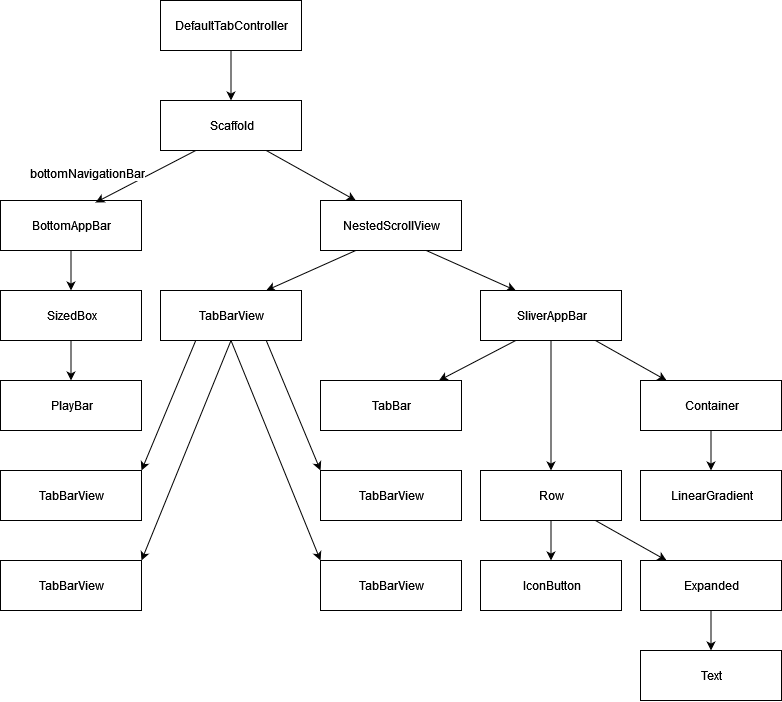
\includegraphics[scale=0.6]{images/Home.png}}
	\caption{Home} 
\end{figure}

The home component is the component shown when the application is first opened.
It is composed of the PlayBar, that allows to control playback and open the
track queue to modify it, and the NestedScrollView, that contains the TabBarView
and the SliverAppBar.

The TabBarView is the widget that shows the available
sections of the music library (TrackList, ArtistList, AlbumList and
PlaylistList).

The SliverAppBar contains the TabBar that actually allows to switch between the
available sections. It also hides itself when the TabBarView is scrolled down
for a sufficient amount.
 

\subsubsection{AlbumList}

\begin{figure}[H]
	\noindent
	\makebox[\textwidth]{ 
		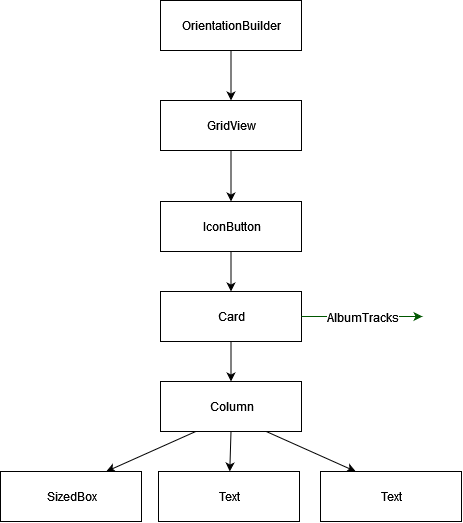
\includegraphics[scale=0.6]{images/AlbumList.png}}
	\caption{AlbumList} 
\end{figure}

This component displays in a grid (GridView) the list of albums (Card) present
on the device. The card contains the cover of the Album, its name and artist.

If a card is tapped (IconButton) the application navigates to the
tracklist of the selected album.

The OrientationBuilder allows to choose an appropriate layout for the device
orientation.

\subsubsection{ArtistList}

\begin{figure}[H]
	\noindent
	\makebox[\textwidth]{ 
		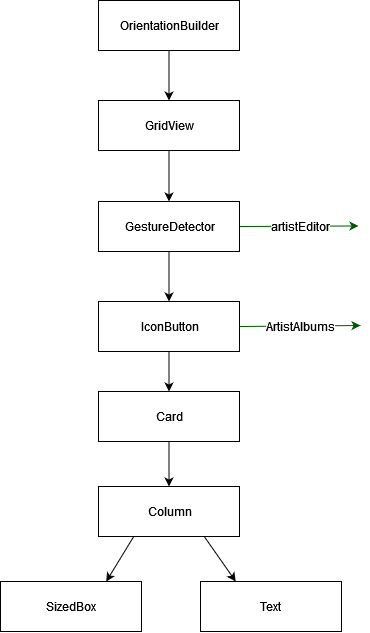
\includegraphics[scale=0.6]{images/ArtistList.png}}
	\caption{ArtistList} 
\end{figure}

This component displays a GridView of the Artist Cards, that contain the artist
name and image. The GestureDetector allows to edit the artist image through
ArtistEditor, while the IconButton allows to access the ArtistAlbum screen.

The OrientationBuilder allows to choose an appropriate layout for the device
orientation.

\subsubsection{PlaylistList}

\begin{figure}[H]
	\noindent
	\makebox[\textwidth]{ 
		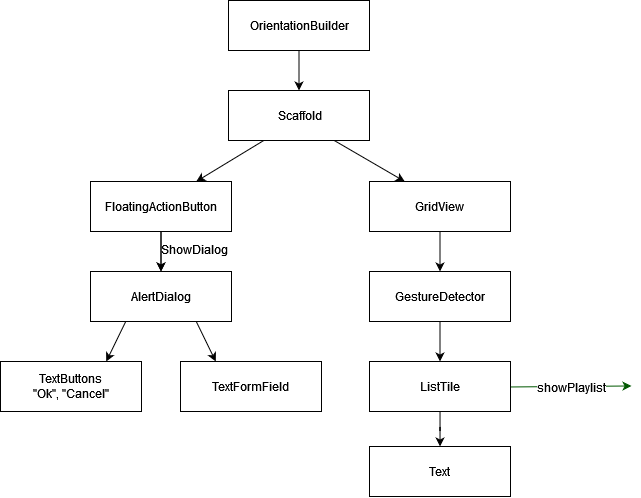
\includegraphics[scale=0.6]{images/PlaylistList.png}}
	\caption{PlaylistList} 
\end{figure}

This component displays a GridView of ListTiles. When tapped, the ListTile
navigates to the ShowPlaylist screen. The GestureDetector detects long presses
and shows accordingly a popup menu to delete the selected playlist if desired.

There is a FloatingActionButton in the bottom right corner of the screen that
allows creating new playlists.

The OrientationBuilder allows to choose an appropriate layout for the device
orientation.

\subsubsection{PlayBar}

\begin{figure}[H]
	\noindent
	\makebox[\textwidth]{ 
		\includegraphics[scale=0.5]{images/PlayBar.png}}
	\caption{PlayBar} 
\end{figure}

The PlayBar contains on the right a button that allow to play or pause music,
depending on current track queue state. On the left there is the description of
the currently playing track, with album cover, track name and artist.

When tapping the track description the application navigates to the PlayingTrack
screen.

\subsubsection{TrackList}

\begin{figure}[H]
	\noindent
	\makebox[\textwidth]{ 
		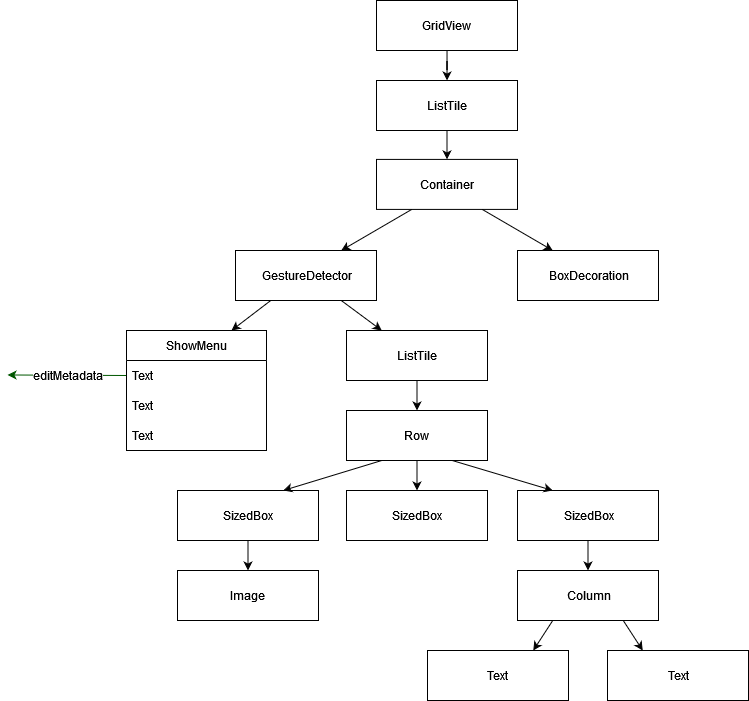
\includegraphics[scale=0.5]{images/TrackList.png}}
	\caption{TrackList} 
\end{figure}

The TrackList is the component that organizes tracks received as argument in a
grid. The grid is composed of GestureDetectors, longtapping which the popup menu
can be opened. 

The menu allows to execute operations on the selected track: view
its metadata, add it to queue or add it to playlist. Instead a short press on
the ListTile brings the user to the PlayingTrack screen and immediately starts
playing the track. 

The ListTile components have on the left the album cover, and
on the left the name and artist of the track.

\subsubsection{ProgressBar}

\begin{figure}[H]
	\noindent
	\makebox[\textwidth]{ 
		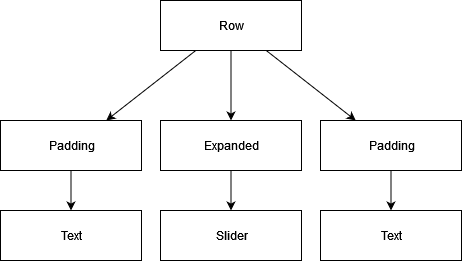
\includegraphics[scale=0.6]{images/ProgressBar.png}}
	\caption{ProgressBar} 
\end{figure}

The ProgressBar is the bar that allows monitoring the progress of the currently
playing track.

It also allows to move the track position forward or backward,
using the Slider. Text at the left side shows the track position, and at the
right shows the track length.

\subsubsection{CoverButton}

\begin{figure}[H]
	\noindent
	\makebox[\textwidth]{ 
		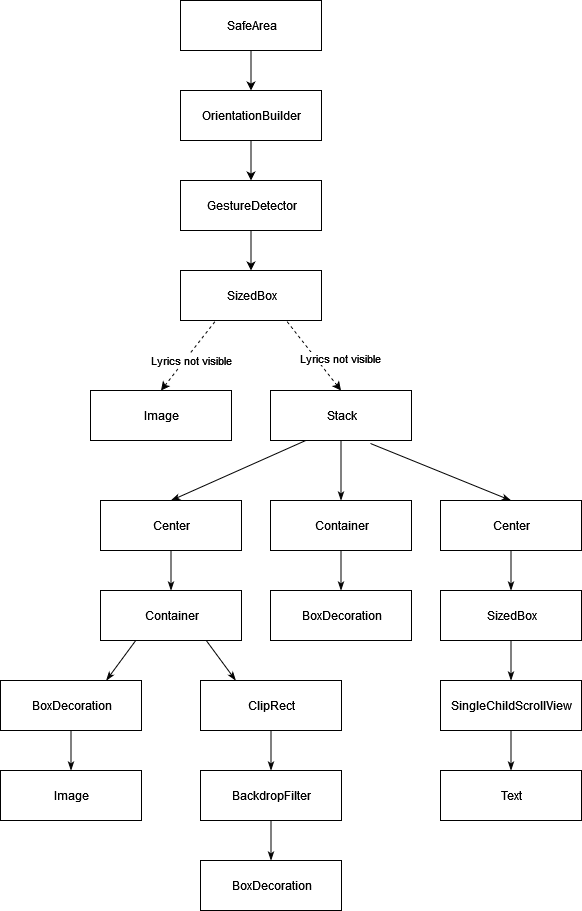
\includegraphics[scale=0.5]{images/CoverButton.png}}
	\caption{CoverButton} 
\end{figure}

The CoverButton is the widget that displays the cover art of an album inside the
PlayingTrack screen. If pressed (GestureDetector), it shows the lyrics
(scrollable Text) of the currently playing track, if available.

The background of the lyrics scroll view is transparent, so that the artwork can
be glimpsed behind them.

The CoverButton is subscribed to the Player, so that whenever a change in the
playing track occurs, that change is shown.

\subsubsection{ArtistEditor}

\begin{figure}[H]
	\noindent
	\makebox[\textwidth]{ 
		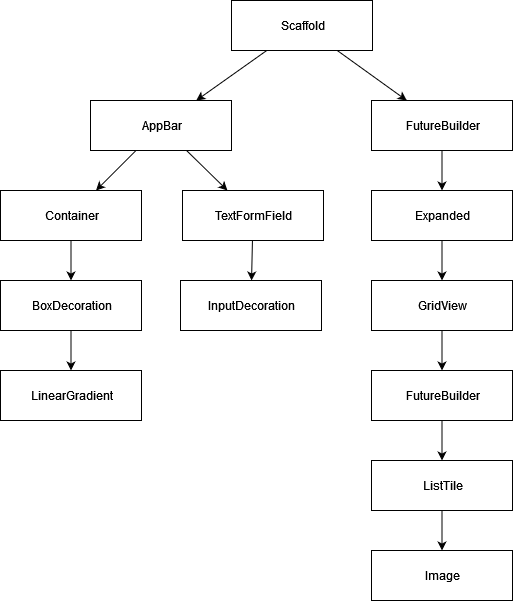
\includegraphics[scale=0.5]{images/ArtistEditor.png}}
	\caption{ArtistEditor} 
\end{figure}

The ArtistEditor is a widget that allows to select a new artwork for the input
artist. The artwork can be searched online by writing inside the TextFormField.

The results, if present, are listed as a grid (GridView) and returned by the
FutureBuilder, as tiles (ListTile) of images and names.

The LinearGradient widget allows to apply a pleasant color to the AppBar.

\subsubsection{MetadataEditor (also known as SearchSong)}

\begin{figure}[H]
	\noindent
	\makebox[\textwidth]{ 
		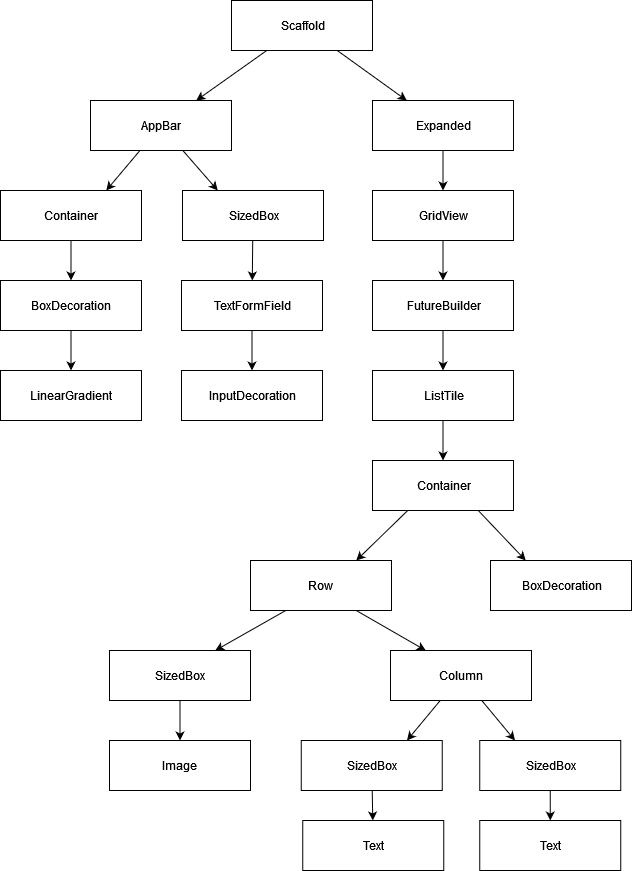
\includegraphics[scale=0.5]{images/MetadataEditor_SearchSong.png}}
	\caption{MetadataEditor (also known as SearchSong)} 
\end{figure}

The MetadataEditor is a widget that allows to set new metadata for the selected
track. The metadata can be searched online by writing inside the TextFormField.

The results, if present are returned as FutureBuilder and listed with a GridView
(this allows for flexible visualization in different orientations). They contain
image, name and artist. If tapped, the metadata of the selected track is
replaced with the metadata of the tapped track.

The LinearGradient widget allows to apply a pleasant color to the AppBar.

\subsubsection{AlbumInfo}

\begin{figure}[H]
	\noindent
	\makebox[\textwidth]{ 
		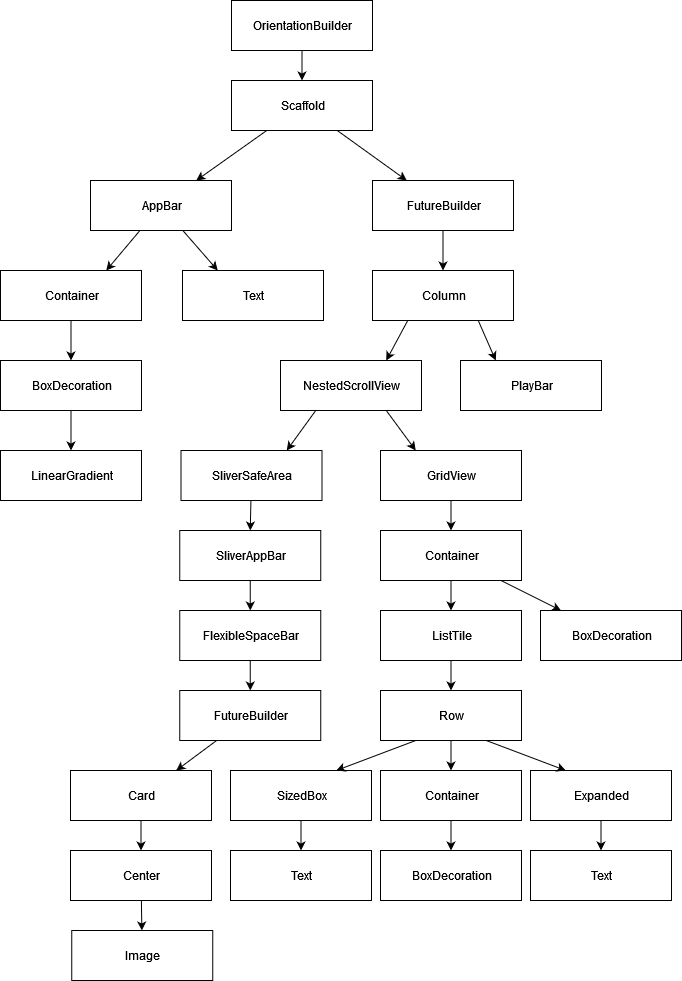
\includegraphics[scale=0.4]{images/AlbumInfo.png}}
	\caption{AlbumInfo} 
\end{figure}

The AlbumInfo screen is composed by the AppBar, the PlayBar and if available
(FutureBuilder), the info about the requested album.

The information about the album is contained in the NestedScrollView. At the top
we have a Card, showing the album cover. The cover will be hidden if scrolling
down the GridView. The grid is composed of tiles with track number and name.

\subsubsection{ArtistInfo}

\begin{figure}[H]
	\noindent
	\makebox[\textwidth]{ 
		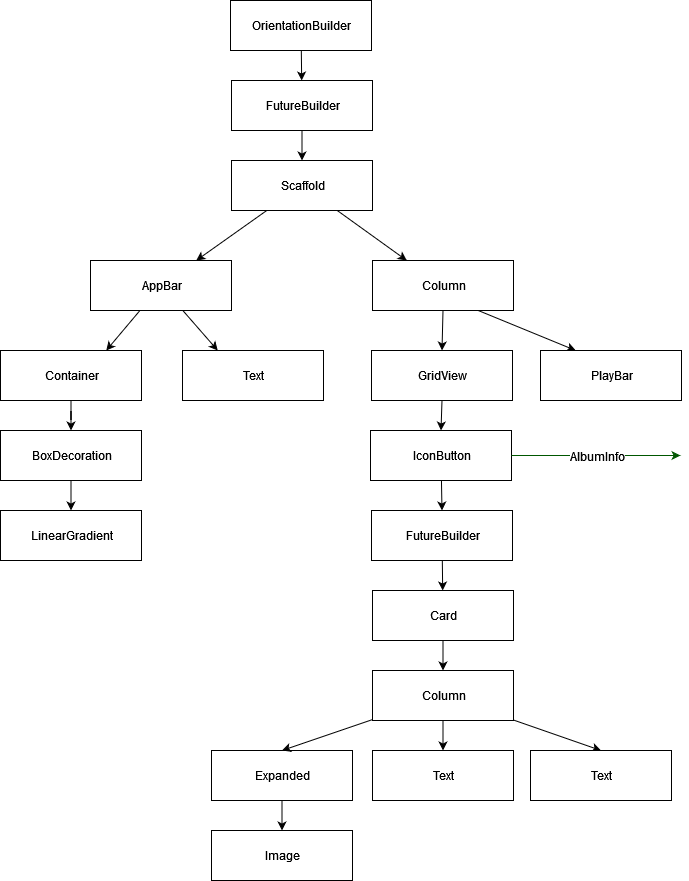
\includegraphics[scale=0.4]{images/ArtistInfo.png}}
	\caption{ArtistInfo} 
\end{figure}

The ArtistInfo screen is composed by the AppBar, the PlayBar and if available
(FutureBuilder), the info about the requested artist.

The information about the artist is contained in the NestedScrollView. The grid
is composed of cards with album image, name and artist.

\subsubsection{AlbumTracks}

\begin{figure}[H]
	\noindent
	\makebox[\textwidth]{ 
		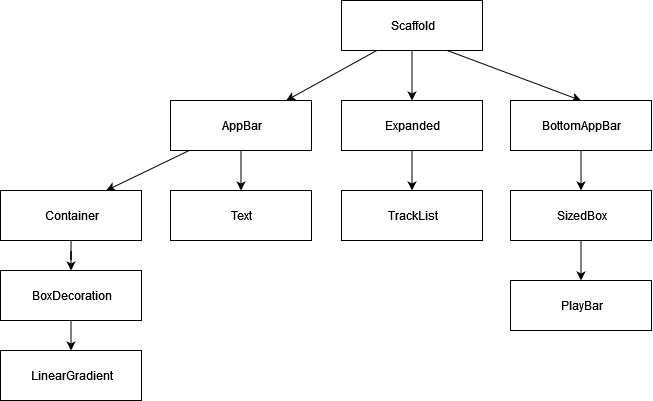
\includegraphics[scale=0.4]{images/AlbumTracks.png}}
	\caption{AlbumTracks} 
\end{figure}

The AlbumTracks screen is composed by the AppBar, the PlayBar and the TrackList.
It receives as input the list of tracks of an album, and displays them in a
grid by using the TrackList.

\subsubsection{ArtistAlbums}

\begin{figure}[H]
	\noindent
	\makebox[\textwidth]{ 
		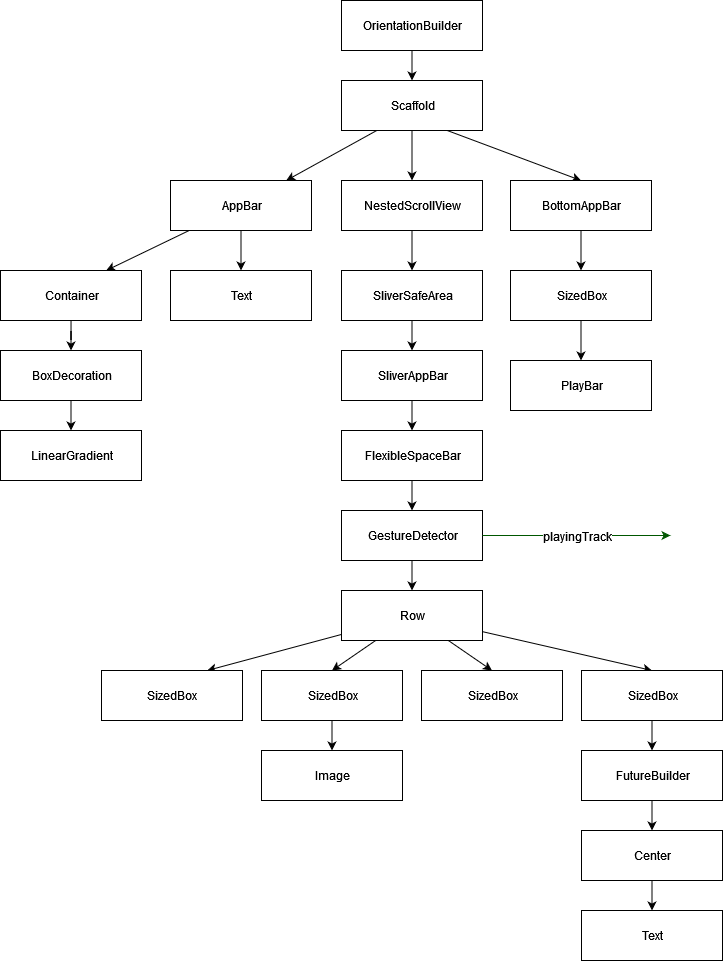
\includegraphics[scale=0.4]{images/ArtistAlbums.png}}
	\caption{ArtistAlbums} 
\end{figure}

TBC.

\end{document}
